
\let\negmedspace\undefined
\let\negthickspace\undefined
\documentclass[journal]{IEEEtran}
\usepackage[a5paper, margin=10mm, onecolumn]{geometry}
\usepackage{tfrupee}
\setlength{\headheight}{1cm}
\setlength{\headsep}{0mm}

\usepackage{gvv-book}
\usepackage{gvv}
\usepackage{cite}
\usepackage{amsmath,amssymb,amsfonts,amsthm}
\usepackage{algorithmic}
\usepackage{graphicx}
\usepackage{textcomp}
\usepackage{xcolor}
\usepackage{txfonts}
\usepackage{listings}
\usepackage{enumitem}
\usepackage{mathtools}
\usepackage{gensymb}
\usepackage{comment}
\usepackage[breaklinks=true]{hyperref}
\usepackage{tkz-euclide}
\usepackage{listings}

\def\inputGnumericTable{}
\usepackage[latin1]{inputenc}
\usepackage{color}
\usepackage{array}
\usepackage{longtable}
\usepackage{calc}
\usepackage{multirow}
\usepackage{hhline}
\usepackage{ifthen}
\usepackage{lscape}
\usepackage{tikz}

\begin{document}

\bibliographystyle{IEEEtran}
\vspace{3cm}

\title{GATE-2015-PH}
\author{EE24BTECH11017-D.KARTHIK}
\maketitle

\renewcommand{\thefigure}{\theenumi}
\renewcommand{\thetable}{\theenumi}
\setlength{\intextsep}{10pt}


\numberwithin{equation}{enumi}
\numberwithin{figure}{enumi}
\renewcommand{\thetable}{\theenumi}

\begin{enumerate}
    \setcounter{enumi}{39}

\item The band gap of an intrinsic semiconductor is $E_g = 0.72 eV \text{ and } m^*_h = 6m^*_e. $ At $300K$, the Fermi level with respect to the valence band $\brak{\text{in } eV}$ is at \rule{1.7cm}{0.2mm} $\brak{\text{upto three decimal places}} k_B = 1.38 x 10^{-23}JK^{-1}$
\item The number of permitted transitions from ${{}^{2}P_{3/2} \rightarrow {}^{2}S_{1/2}}
$ in the presence of a weak magnetic field is \rule{3cm}{0.2mm}
\item Which one of the following represents the electron occupancy for a superconductor in its normal and superconducting states?
\textbf{
diagrams
}
\begin{multicols}{2}
\begin{enumerate}

    \item 
\resizebox{0.3\textwidth}{!}{%
\begin{circuitikz}
\tikzstyle{every node}=[font=\LARGE]
\draw [->, >=Stealth] (9.5,6.5) -- (9.5,11.5);
\draw [->, >=Stealth] (9.5,6.5) -- (15.5,6.5);
\draw [short] (10,11) .. controls (10.25,8.75) and (8.75,6.25) .. (12.5,7);
\node [font=\LARGE] at (14.5,6) {E};
\node [font=\LARGE] at (9.5,12.5) {Superconducting state};

\node [font=\LARGE] at (8,10) {f\brak{E}};
\draw [->, >=Stealth] (3,6.5) -- (9,6.5);
\draw [->, >=Stealth] (3,6.5) -- (3,12);
\draw [short] (3,9.5) -- (6.5,9.5);
\draw [short] (6.5,9.5) -- (6.5,6.5);
\node [font=\LARGE] at (2.75,12.75) {Normal mode};
\node [font=\LARGE] at (8,5.75) {E};
\node [font=\LARGE] at (2.25,9.75) {f\brak{E}};
\end{circuitikz}
}%

    \item \input{fig/2.tex}
    \item 
\resizebox{0.38\textwidth}{!}{%
\begin{circuitikz}
\tikzstyle{every node}=[font=\large]
\draw [->, >=Stealth] (3.5,8.5) -- (3.5,11);
\draw [->, >=Stealth] (3.5,8.5) -- (6.25,8.5);
\draw (3.5,10) to[short] (4.75,10);
\node [font=\large] at (3.5,11.5) {Normal state};
\draw [short] (5,9.75) .. controls (5.25,8.75) and (5.25,8.75) .. (5.75,8.5);
\draw [short] (4.75,10) .. controls (5,10) and (5,10) .. (5,9.75);
\node [font=\Large] at (5.5,8) {E};
\node [font=\LARGE] at (3,10) {};
\node [font=\Large] at (2.5,10) {$f\brak{E}$};
\draw [->, >=Stealth] (8.5,8.5) -- (11.25,8.5);
\draw [->, >=Stealth] (8.5,8.5) -- (8.5,11);
\draw [short] (8.5,9.75) -- (10.25,9.75);
\draw [short] (10.25,9.75) -- (10.25,8.5);
\node [font=\large] at (8.5,11.5) {Superconducting State};
\node [font=\large] at (10.75,8) {E};
\node [font=\large] at (7.25,9.75) {f\brak{E}};
\end{circuitikz}
}%

    
    \item \resizebox{0.35\textwidth}{!}{%
\begin{circuitikz}
\tikzstyle{every node}=[font=\LARGE]
\draw [->, >=Stealth] (3,6) -- (3,10.75);
\draw [->, >=Stealth] (3,6) .. controls (5.5,6) and (5.5,6) .. (7.75,6) ;
\draw (3,8) to[short] (4.75,8);
\node [font=\LARGE] at (2.75,11.25) {Superconducting state};
\draw [short] (5.25,7.25) .. controls (5.5,6.25) and (5.5,6.25) .. (6,6);
\draw [short] (4.75,8) .. controls (5.25,8) and (5,7.75) .. (5.25,7.25);
\node [font=\LARGE] at (7.25,5.5) {E};
\node [font=\LARGE] at (2.5,8.5) {};
\node [font=\LARGE] at (1.75,9.75) {f\brak{E}};
\draw [->, >=Stealth] (10,6) -- (10,11);
\draw [->, >=Stealth] (10,6) -- (16,6);
\draw [short] (10.5,10.5) .. controls (10.75,8.25) and (9.25,5.75) .. (13,6.5);
\node [font=\LARGE] at (15,5.5) {E};
\node [font=\LARGE] at (10,12) {Normal state};
\node [font=\LARGE] at (8.5,9.5) {f\brak{E}};
\end{circuitikz}
}%
\end{enumerate}
\end{multicols}






\item A charge $-q$ is distributed uniformly over a sphere, with a positive charge $q$ at its center in $\brak{i}$. Also in $\brak{ii}$, a charge $-q$ is distributed uniformly over an ellipsoid with a positive charge $q$ at its center. With respect to the origin of the coordinate system, which one of the following statements is correct?
\begin{centering}
\resizebox{0.6\textwidth}{!}{%
\begin{circuitikz}
\tikzstyle{every node}=[font=\large]

% Circle with gray fill
\draw[fill=gray!30] (5.75,11.25) circle (1.5cm);
\draw[->, >=Stealth] (5.75,11.25) -- (5.75,14);
\draw[->, >=Stealth] (5.75,11.25) -- (9.75,11.25);
\draw[->, >=Stealth] (5.75,11.25) -- (3.75,8.75);
\node[font=\Large] at (6,14) {X};
\node[font=\Large] at (9,11) {Z};
\node[font=\Large] at (4.5,9) {Y};
\node[font=\Large] at (5.5,8) {\brak{i}};

% Ellipse with gray fill
\draw[fill=gray!30] (15.75,11.5) ellipse (2cm and 1cm);
\draw[->, >=Stealth] (15.75,11.5) -- (15.75,13.75);
\draw[->, >=Stealth] (15.75,11.5) -- (20.75,11.5);
\draw[->, >=Stealth] (15.75,11.5) -- (14,9);
\node[font=\Large] at (15.75,14) {X};
\node[font=\Large] at (20,11) {Z};
\node[font=\Large] at (15,9.5) {Y};
\node[font=\Large] at (16,8) {\brak{ii}};

\end{circuitikz}
}%
\end{centering}
\begin{enumerate}
    \item The dipole moment is zero in both $\brak{i}$ and $\brak{ii}$
    \item The dipole moment is non-zero in $\brak{i}$ but zero in $\brak{ii}$
    \item The dipole moment is zero in $\brak{i}$ but non-zero in $\brak{ii}$
    \item The dipole moment is non-zero in both $\brak{i}$ and $\brak{ii}$
\end{enumerate}
\item Consider the circuit shown in the figure, where $RC = 1$. For an input signal $V_1$ shown below, choose the correct $V_o$ from the options:\\
\begin{figure}[!ht]
\centering
\resizebox{1\textwidth}{!}{%
\begin{circuitikz}
\tikzstyle{every node}=[font=\Large]
\draw (8.75,10) to[short, -o] (10,10) ;
\draw (9.25,10) to[short] (9.25,11.5);
\draw (9.25,11.5) to[R] (7.25,11.5);
\draw (7.25,11.5) to[short] (6.75,11.5);
\draw (6.75,11.5) to[short] (5.5,11.5);
\draw (6.25,10.5) to[short] (4.75,10.5);
\draw (5.5,11.5) to[short] (5.5,10.5);
\draw (6.25,9.5) to[short] (5.5,9.5);
\draw (5.5,9.5) to[R] (5.5,7.75);
\draw (5.5,7.75) to (5.5,7.5) node[ground]{};
\draw (4.75,10.5) to[C] (3.75,10.5);
\draw (3.75,10.5) to[short, -o] (3,10.5) ;
\node [font=\Large] at (8,12) {R};
\node [font=\Large] at (5,8.5) {R};
\node [font=\Large] at (5,8.5) {};
\node [font=\Large] at (4.25,11) {C};
\node [font=\Large] at (2.5,10.5) {$v_i$};
\node [font=\Large] at (10.5,10) {$v_o$};
\draw (7.75,10) node[op amp,scale=1, yscale=-1 ] (opamp2) {};
\draw (opamp2.+) to[short] (6.25,10.5);
\draw  (opamp2.-) to[short] (6.25,9.5);
\draw (8.95,10) to[short](9.25,10);
\draw (7.75,10) node[op amp,scale=1] (opamp2) {};
\draw (opamp2.+) to[short] (6.25,9.5);
\draw  (opamp2.-) to[short] (6.25,10.5);
\draw (8.95,10) to[short](9.25,10);
\draw [->, >=Stealth] (13.75,8.5) -- (13.75,12);
\draw [->, >=Stealth] (13.75,8.5) -- (21,8.5);
\foreach \x in {0,...,1}{
  \draw  (13.75+\x*2.941176470588235,8.5) -- ++(1.4705882352941175,2.1) -- ++ (1.4705882352941175, -2.1);
}
\draw [dashed] (18.25,10.5) -- (13.5,10.5);
\draw [dashed] (15.25,10.75) -- (15.25,8.5);
\draw [dashed] (18.25,10.75) -- (18.25,8.5);
\node [font=\Large] at (15.25,8.25) {1};
\node [font=\Large] at (16.75,8.25) {2};
\node [font=\Large] at (18.25,8.25) {3};
\node [font=\Large] at (20.75,8) {t};
\node [font=\Large] at (13.5,10.5) {1};
\node [font=\Large] at (13.25,12) {$v_i$};
\end{circuitikz}
}%

\label{fig:my_label}
\end{figure}
\begin{multicols}{2}
\begin{enumerate}
   \item \begin{tikzpicture}
   
    \draw[->, >=Stealth, thick] (0, 0) -- (5, 0) node[below] {$t$};
    \draw[->, >=Stealth, thick] (0, -1.5) -- (0, 2) node[left] {$V_o$};
    \draw[thick] (0, -1) -- (1, -1);  
    \draw[thick] (1, -1) -- (1, 1);   
    \draw[thick] (1, 1) -- (2, 1);    
    \draw[thick] (2, 1) -- (2, -1);                                
    \draw[thick] (2, -1) -- (3, -1);  
    \draw[thick] (3, -1) -- (3, 1);   
    \draw[thick] (3, 1) -- (4, 1);    
    \draw[thick] (4, 1) -- (4, -1);   
    \draw[thick] (4, -1) -- (5, -1);      
    \node at (1.1, -0.3) {1};
    \node at (2.1, -0.3) {2};
    \node at (3.1, -0.3) {3};
    \node at (-0.3, 1) {1};
    \node at (-0.3, -1) {-1};
\end{tikzpicture}


  \item \begin{tikzpicture}
    \draw[->] (-0.5,0) -- (4.2,0) node[right] {$t$};
    \draw[->] (0,-0.5) -- (0,2) node[above] {$V_0$};

    % Markings on the axes
    \foreach \x in {1,2,3} {
        \draw (\x,0.1) -- (\x,-0.1) node[below] {$\x$};
    }
    \draw (-0.1,1) -- (0.1,1) node[left] {$1$};

    % Triangular waveform
    \draw (0,0) -- (1,1) -- (2,0) -- (3,1) -- (4,0);

    % Dashed lines for clarity
    \draw[dashed] (1,0) -- (1,1);
    \draw[dashed] (3,0) -- (3,1);
\end{tikzpicture}
   \columnbreak
    \item \input{fig/c.tex} 
   \item \resizebox{0.45\textwidth}{!}{%
\begin{circuitikz}
\tikzstyle{every node}=[font=\Large]
\draw [->, >=Stealth] (6.25,6.75) -- (6.25,12.5);
\draw [->, >=Stealth] (6.25,8.75) -- (16.25,8.75);
\foreach \x in {0,...,1}{
  \draw  (6.25+\x*3.846153846153846,7.5) -- ++(0,2.6) -- ++ (1.923076923076923, 0) -- ++(0, -2.6) -- ++(1.923076923076923,0);
}
\draw [short] (14,7.5) -- (14,10);
\node [font=\Large] at (6,10) {1};
\node [font=\Large] at (5.75,7.5) {-1};
\node [font=\Large] at (8.5,8.5) {1};
\node [font=\Large] at (10.25,8.5) {2};
\node [font=\Large] at (12.25,8.5) {3};
\node [font=\Large] at (16,8.5) {t};
\node [font=\Large] at (5.75,12.25) {$V_o$};
\end{circuitikz}
}%
      
    
\end{enumerate}
    
\end{multicols}


\item A long solenoid is embedded in a conducting medium and is insulated from the medium. If the current through the solenoid is increased at a constant rate, the induced current in the medium as a function of the radial distance $r$ from the axis of the solenoid is proportional to
\begin{multicols}{2}
\begin{enumerate}
    \item $r^2$ inside the solenoid and $\frac{1}{r}$ outside
    \item $r$ inside the solenoid and $\frac{1}{r^2}$ outside
 \item $r^2$ inside the solenoid and $\frac{1}{r^2}$ outside
  \item $r$ inside the solenoid and $\frac{1}{r}$ outside
\end{enumerate}
\end{multicols}
\item In the simple current source in the figure, $Q_1 \text{ and } Q_2$ are identical transistors with current gain $\beta = 100$ and $V_{BE} = 0.7 V$\\
\begin{figure}[!ht]
\centering
\resizebox{0.3\textwidth}{!}{%
\begin{circuitikz}
\tikzstyle{every node}=[font=\Large]
\draw (6.75,13.5) to[short, -o] (6.75,14.25) ;
\draw (6.75,13.5) to[R] (6.75,11.75);
\draw (6.75,11.75) to[Tnpn, transistors/scale=1.19] (6.75,9.75);

\draw (7.75,10.75) to[short] (8.75,10.75);
\draw (6.75,11.75) to[short] (8.25,11.75);
\draw (8.25,11.75) to[short] (8.25,10.75);
\draw (9.5,11.5) to[short, -o] (9.5,12.5) ;
\draw (9.5,9.75) to[Tnpn, transistors/scale=1.19] (9.5,11.75);
\draw (9.5,9.75) to (9.5,9.5) node[ground]{};
\draw (6.75,9.75) to[short] (9.5,9.75);
\node [font=\large] at (6.5,10.75) {$Q_1$};
\node [font=\large] at (9.5,10.75) {$Q_2$};
\node [font=\Large] at (10,12.5) {$I_o$};
\node [font=\large] at (6.5,14.75) {$V_{cc}=30V$};
\node [font=\large] at (6,12.75) {5k$\Omega$};
\draw [->, >=Stealth] (9.75,12.5) -- (9.75,12);
\end{circuitikz}
}%
 \captionsetup{labelformat=empty} % This removes "Figure" and number
\caption{The cuurent $I_0 \brak{\text{in $mA$}}$ is \rule{1.7cm}{0.2mm} $\brak{\text{upto two decimal places}}$}
\end{figure}

\item {Match the phrases in Group I and Group II and identify the correct option.}
\begin{table}[ht]
\centering
\begin{tabular}{ll}

\textbf{Group I} & \textbf{Group II} \\

(P) Electron spin resonance (ESR) & (i) radio frequency \\
(Q) Nuclear magnetic resonance (NMR) & (ii) visible range frequency \\
(R) Transition between vibrational states of a molecule & (iii) microwave frequency \\
(S) Electronic transition & (iv) far-infrared range   
 \\

\end{tabular}

\label{tab:matching_table}
\end{table}
\begin{multicols}{2}
\begin{enumerate}
\item  (P-i), (Q-ii), (R-iii), (S-iv)
\item  (P-ii), (Q-i), (R-iv), (S-iii)
\item  (P-iii), (Q-iv), (R-i), (S-ii)
\item  (P-iii), (Q-i), (R-iv), (S-ii)
\end{enumerate}
\end{multicols}
\item Consider the motion of the Sun with respect to the rotation of the Earth about its axis. If $\vec{\overrightarrow{F_c}}$ and $\vec{\overrightarrow{F}{_{Co}}}$ denote the centrifugal and the Coriolis forces, respectively, acting on the Sun, then
\begin{enumerate}
    \item $\vec{\overrightarrow{F_c}}$ is radially outward and $\vec{\overrightarrow{F}{_{Co}}} = \vec{\overrightarrow{F_c}}$
        \item $\vec{\overrightarrow{F_c}}$ is radially inward and $\vec{\overrightarrow{F}{_{Co}}} = \vec{-2\overrightarrow{F_c}}$
         \item $\vec{\overrightarrow{F_c}}$ is radially outward and $\vec{\overrightarrow{F}{_{Co}}} = \vec{-2\overrightarrow{F_c}}$
          \item $\vec{\overrightarrow{F_c}}$ is radially outward and $\vec{\overrightarrow{F}{_{Co}}} = \vec{2\overrightarrow{F_c}}$
\end{enumerate}
\item In a rigid-rotator of mass $M$, if the energy of the first excited state is $1 meV$, then the fourth excited state energy $\brak{\text{in } meV}$ is \rule{1.7cm}{0.2mm}
\item $\text{A plane wave } \brak{\hat{x} + i\hat{y}}\vec{E}_0 \exp[i(kz - \omega t)] \text{ after passing through an optical element emerges as}
\brak{\hat{x} - \hat{iy}}\vec{E}_0 \exp[i(kz - \omega t)], \text{ where } k \text{ and } \omega \text{ are the wavevector and the angular frequency,}
\text{respectively. The optical element is a }$
\begin{multicols}{2}
\begin{enumerate}
    \item quarter wave plate
    \item half wave plate
    \item polarizer
    \item Faraday rotator
\end{enumerate}
\end{multicols}
\item The Lagrangian for a particle of mass $m$ at a position $\vec{\overrightarrow{r}}$ moving with a velocity $\vec{\overrightarrow{v}}$ is given by $L = \frac{m}{2}\vec{\overrightarrow{v}^2} + C\vec{\overrightarrow{r}.\vec{\overrightarrow{v} - V\brak{r}}}$, where $V\brak{r}$is a potential and $C$ is a constant. If $\vec{\overrightarrow{p}{_c}}$ is the canonical momentum, then its Hamiltonian is given by
\begin{multicols}{2}
\begin{enumerate}
    \item $\frac{1}{2m}\brak{\vec{\overrightarrow{p}_c} + C\vec{\overrightarrow{r}}}^2 + V\brak{r}$
    \item $\frac{1}{2m}\brak{\vec{\overrightarrow{p}_c} - C\vec{\overrightarrow{r}}}^2 + V\brak{r}$
    \item $\frac{p_c^2}{2m} + V\brak{r}$
    \item $\frac{1}{2m}p_c^2 + C^2r^2 + V\brak{r}$
\end{enumerate}
\end{multicols}
\item The Hamiltonian for a system of two particles of masses $m_1$ and $m_2$ at $\vec{\overrightarrow{r}{_1}}$ and $\vec{\overrightarrow{r}{_2}}$ having velocities $\vec{\overrightarrow{v}{_1}}$ and $\vec{\overrightarrow{v}{_2}}$ is given by $H = \frac{1}{2}m_1v_1^2 + \frac{1}{2}m_2v_2^2 + \frac{C}{\brak{\vec{\overrightarrow{r}{_1} - \vec{\overrightarrow{r}{_2}}}}^2}\hat{z}.\brak{\vec{\overrightarrow{r}{_1}}\times\vec{\overrightarrow{r}{_2}}}$,where $C$ is a constant. Which one of the following statements is correct?
\begin{enumerate}
    \item The total energy and total momentum are conserved 
    \item Only the total energy is conserved
    \item Only the total energy and the $z-$component of the total angular momentum are conserved 
    \item The total energy and total angular momentum are conserved
\end{enumerate}

\end{enumerate}

 


\end{document}